\section{Energy Procurement in Illinois}
\label{section:markets}

This section describes the ways consumers and municipalities procure electricity
in Illinois. This brief interlude provides essential context for understanding
the structural barriers preventing municipalities from taking advantage of
energy modeling tools to aid planning and elucidates the frequently limited
scope of municipal energy plans. Figure \ref{fig:illinois-flow-chart} provides a
visual guide for electricity procurement from the perspective of an individual
consumer with arrows indicating directional relationships.

First, Illinois belongs to two \acp{rto}, \ac{pjm} and \ac{miso}, which conduct
wholesale energy auctions through which market participants purchase
electricity. Residential customers do not participate directly in the open energy
market. Instead, they interface with a utility or municipality that procures
electricity on their behalf. Some municipalities, such as Naperville, own their
own utilities. Second, Illinois restructured its electricity market in 1997,
prohibiting \aclp{iou} from owning both transmission infrastructure and
generating infrastructure \cite{illinois_90th_general_assembly_electric_1997}.
This means that \acp{iou} must purchase electricity on the open market rather
than having in-house generation. Municipally-owned utilities are exempt from
this rule. Finally, the deregulation of Illinois' electricity market limits the
state legislature's ability to force the construction of new generation or the
retirement of old generation. The legislature can direct the \ac{ipa} to procure
a certain amount of generation from specific generators and the legislature may
enact policies which incentivize desirable generators to come to Illinois.


\begin{figure}[ht!]
    \centering
    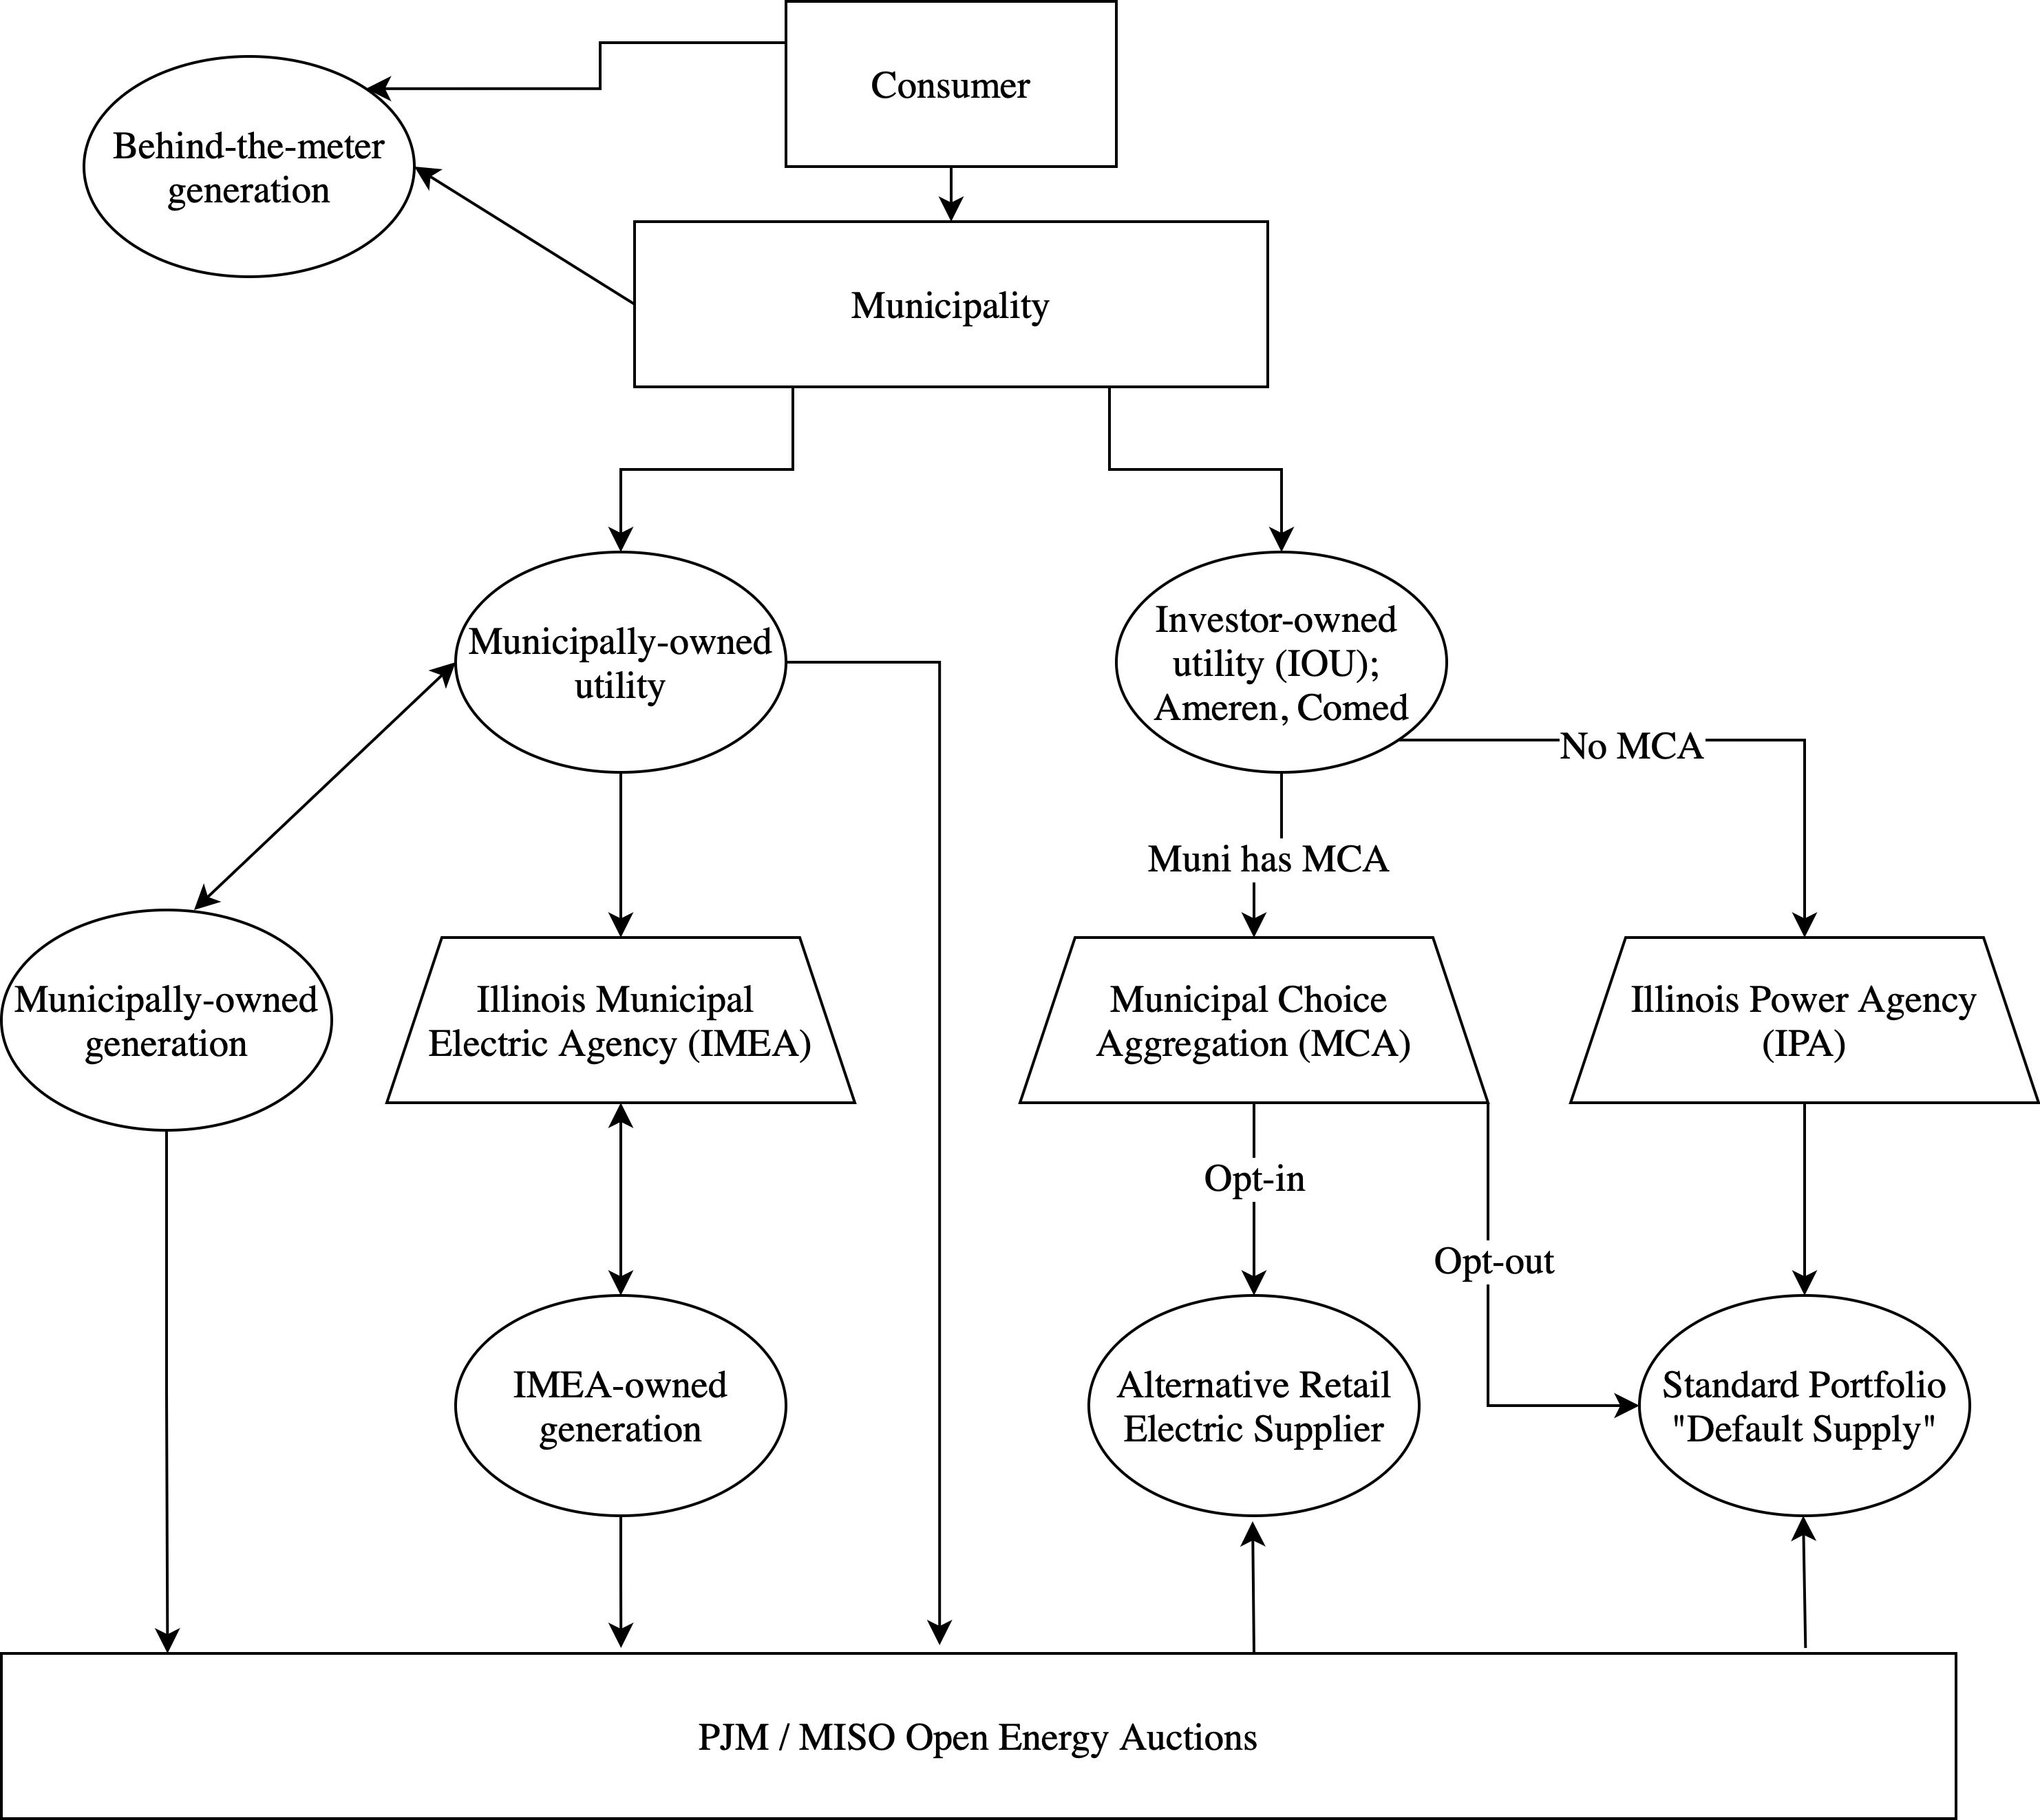
\includegraphics[width=0.9\columnwidth]{figures/07_interview_chapter/illinois-electric-choice.png}
    % 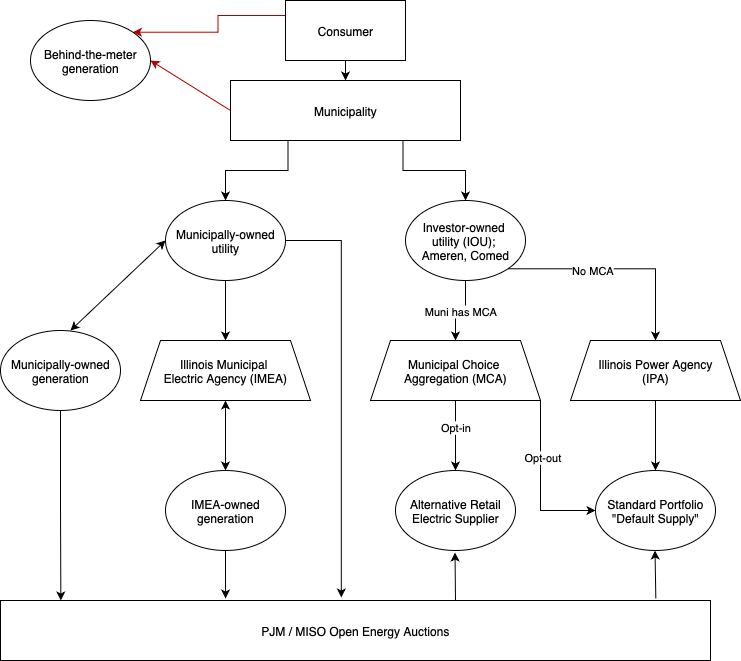
\includegraphics[width=0.9\columnwidth]{figures/07_interview_chapter/illinois-electric-choice.drawio.png}
    % \resizebox{0.75\columnwidth}{!}{\input{figures/07_interview_chapter/illinois-electric-choice.drawio.svg}}
    \caption{A flow chart describing how consumers may procure electricity in
    Illinois. 
    % \textcolor{red}{!! NOT FINAL !!}
    }
    \label{fig:illinois-flow-chart}
\end{figure}

Figure \ref{fig:illinois-flow-chart} shows consumers residing within
municipalities. Municipalities that own and operate a utility may obtain
electric supply by owning electric generation, participating in the energy
market, or contracting with another organization, such as the \ac{imea}, to
handle the supply procurement. In turn, \ac{imea} can procure energy by owning
generating capacity or through the energy market. Most municipalities in
Illinois are served by one of the two major \acp{iou}, Ameren or ComEd. Due to
the Public Utilities Act of 1997, these utilities cannot profit from the supply of
electricity \cite{illinois_90th_general_assembly_electric_1997}. Rather, their
customers (consumers or municipalities) direct the utility to supply electricity
from a chosen supplier. If customers do not choose a supplier, they will receive
the default supply, procured by the \ac{ipa}. In Illinois, consumers can opt for
their municipality (where allowed) to negotiate electricity prices on their
behalf through \ac{mca}. Municipalities may either select from an \ac{ares} or
choose the default supply.\footnote{An \ac{ares} is an entity certified by the
\ac{icc} that sells electricity to customers. This electricity is generated
through privately owned resources or through purchases from the electricity
market.} Although not depicted in Figure \ref{fig:illinois-flow-chart},
consumers who reside in a municipality without \ac{mca} may still choose to
purchase electricity supply from an \ac{ares} as an individual. Of course,
consumers and municipalities may, where permitted, obtain energy by investing in
\ac{btm} resources, commonly rooftop solar panels or batteries. Municipalities
that currently outsource their electricity procurement to \ac{imea} are
contractually prohibited from building certain \ac{btm} resources.

\FloatBarrier